% =====================================================================
%  Airway segmentation and anatomical branch assignment in pediatric CT
%  LNCS / MICCAI format. Submission version.
%
%  The long working document, which carries the full derivations, every
%  table and all open questions, is airway_method_paper_FULL_working.tex.
%  Detail belongs there, or in a supplement if one is submitted, not here.
%
%  Style rules: no em dashes, no semicolons in body prose.
%  Compile: tectonic -X compile airway_method_paper.tex
% =====================================================================
\documentclass[runningheads]{llncs}

\usepackage{graphicx}
\usepackage{booktabs}
\usepackage{array}
\usepackage{makecell}
\usepackage{amsmath}
\usepackage{amssymb}
\usepackage{xcolor}
\usepackage[hidelinks]{hyperref}
\usepackage{tikz}
\usetikzlibrary{arrows.meta,positioning,fit,backgrounds,calc}
\renewcommand\UrlFont{\color{blue}\rmfamily}

% A small stretch allowance keeps the narrow LNCS measure from overflowing
% rather than forcing awkward rewrites of otherwise correct sentences.
\setlength{\emergencystretch}{1em}

\newcommand{\todo}[1]{\textcolor{gray}{\textit{[#1]}}}

% Block diagram styles. Fills are light so that the labels stay legible after
% the page reduction, and the two stages of the pipeline are separated by fill
% rather than by a box, which would cost vertical space.
\definecolor{segfill}{HTML}{DCE9F7}
\definecolor{segline}{HTML}{2A78D6}
\definecolor{labfill}{HTML}{E6E0F5}
\definecolor{labline}{HTML}{6B4FBB}
\definecolor{iofill}{HTML}{ECECE8}
\tikzset{
  blk/.style={draw, rounded corners=2pt, align=center, inner sep=3.2pt,
              font=\scriptsize, minimum height=7.5mm, line width=0.5pt},
  seg/.style={blk, fill=segfill, draw=segline},
  lab/.style={blk, fill=labfill, draw=labline},
  io/.style={blk, fill=iofill, draw=black!55},
  op/.style={draw, circle, inner sep=0.8pt, font=\scriptsize, line width=0.5pt,
             fill=segfill, draw=segline},
  fl/.style={-{Latex[length=1.6mm,width=1.4mm]}, line width=0.5pt, draw=black!70},
  note/.style={font=\tiny, text=black!60, align=center},
}
\newcommand{\hd}[1]{\makecell[c]{#1}}

\begin{document}

\title{Airway Segmentation and Anatomical Branch Assignment\\in Pediatric Chest CT}
\titlerunning{Pediatric airway segmentation and branch assignment}

% ANONYMOUS FOR REVIEW. The real block is kept below so it can be restored in
% one edit. The marker meanings are assumed and need confirming: star for equal
% first authorship, double star for equal senior authorship, dagger for the
% corresponding author.
%
% \author{%
% Huseyin Umut Isik\inst{1}\textsuperscript{$\star$} \and
% Ege Mert Balcik\inst{1}\textsuperscript{$\star,\dagger$} \and
% Sila Kurugol\inst{3}\textsuperscript{$\star\star$} \and
% \c{S}eyda Ertekin\inst{1,2}\textsuperscript{$\star\star$}}
% \authorrunning{H. U. Isik et al.}
% \institute{Department of Computer Engineering, METU, Ankara, Turkey \and
% METU-DTX Digital Transformation and Innovation Center, Ankara, Turkey \and
% Quantitative Intelligent Imaging Lab, Boston Children's Hospital and Harvard
% Medical School, Boston, MA, USA}
%
% Restoring the block above also means restoring the marker footnote that used
% to follow \maketitle, and the acknowledgement and funding text.
\author{Anonymous}
\authorrunning{Anonymous}
\institute{Paper submitted for blind review}

\maketitle

\begin{abstract}
A segmented airway tree answers few clinical questions until its branches are
named, and the methods that segment airways and the recent work that names them
are developed and validated almost entirely in adults. For an automated method
the pediatric airway is not a smaller version of the adult one. Branch calibre
approaches the voxel size, one model has to cover the range of physical sizes
between a newborn and an adolescent, and acquisition is lower dose and often
without breath hold. These differences change how a method fails rather than
only how well it scores. We combine three public airway models by union and
retain a single connected component chosen by a seed rather than by size, then
name every branch with a graph transformer that had to be trained here because
its weights were never released. Evaluation covers a public adult benchmark,
public branch-wise anatomical labels, and nine expert-annotated volumes from a
balanced pediatric cohort spanning birth to adolescence. Combining models is
worth far more in children than in adults. It raises the percentage of reference
branches detected by 6.0 points over the best pair of models, where the same
gain on the adult benchmark is 0.7. Retaining
the largest connected component instead of the seeded one destroys the airway
silently, and every pediatric examination where it does so is an infant under
one year. Segmentation accuracy falls steeply with depth while naming accuracy
stays near flat, so branch recovery rather than naming is what limits the
pipeline.

\keywords{Airway segmentation \and Anatomical labelling \and Pediatric chest CT
\and Model ensemble.}
\end{abstract}

% =====================================================================
\section{Introduction}
\label{sec:intro}

Most questions asked of an airway tree are asked about a particular branch. A
bronchoscopist needs the segmental bronchus that leads to a lesion, a
radiologist reporting bronchiectasis needs the affected lobe and segment, and a
morphometric study needs the same anatomical branch across subjects. A binary
mask supports none of these on its own. Anatomical labelling is therefore a second task on top of
segmentation, and recent work addresses it at lobar, segmental and subsegmental
resolution \cite{zhang2025airmorph}.

That work, and the segmentation methods it builds on \cite{carmo2024medpseg,wu2025tfenet}, was developed and validated in adults. The pediatric airway
differs in ways that matter for an automated method. Calibre relative to voxel
size is smaller, so a mid-generation bronchus in an infant may span only a few
voxels and the partial-volume boundary becomes a large fraction of the
structure. One model must cover a range of physical sizes an adult model never
sees, and acquisition is lower dose and often without breath hold.

These differences change how a method fails rather than only how well it scores.
A permissive network produces spurious structures, and in a small airway such a
structure can exceed the true tree in volume, at which point the routine step of
retaining the largest connected component discards the airway and keeps the
artefact. The failure is silent, because the retained object still resembles an
airway tree, and whole-tree accuracy conceals it because the proximal
generations carry most of the voxels while the peripheral generations are
exactly those most affected by resolution.

\smallskip\noindent\textbf{Contributions.}
(i) A branch assignment stage for the pediatric airway tree, following the
architecture of \cite{zhang2025airmorph}, whose weights were never released and
whose description is incomplete, so the training procedure was reconstructed
here with every open choice stated explicitly. (ii) An ensemble segmentation
front end with a seeded component-selection rule that removes the silent failure
above. (iii) A generation-limited evaluation protocol for settings where an
exhaustive expert reference is unattainable. (iv) A pediatric benchmark of the
segmentation front end on nine expert-annotated volumes, with the bias its
annotation provenance introduces measured and stated. We make no claim of superiority
over state-of-the-art segmentation models and report no such comparison.

% =====================================================================
\section{Data}
\label{sec:data}

\textbf{Public benchmark.} The binary airway segmentation task of the Airway
Tree Modeling challenge \cite{atm22} provides 299 annotated thoracic CT
volumes, partitioned
once with a fixed seed into 239 training, 30 validation and 30 test volumes.
Every benchmark value below is computed on the 30 test volumes, which were
withheld from all development.

\textbf{Anatomical labels.} A second annotation set covers 118 of those volumes
with branch-wise anatomical labels. The 11 that also fall in the segmentation
test set were reserved as the labelling test split and the remaining 107
supplied labelling training and validation, so no volume used to evaluate
labelling contributed to training either stage.

\textbf{Pediatric cohort.} Ninety examinations from 90 distinct patients aged
0.2 to 18.0 years, drawn by integer programming from two processed cohorts, with
exactly ten examinations in each of nine two-year age bands, at most one scan per
patient, and sex recorded for all. The cohort is 43 male and 47 female. Where a
result is reported on the larger screened pool rather than the balanced cohort,
83 examinations, this is stated. Nine of these examinations carry an expert
airway annotation, drawn by three annotators.
\todo{IRB approval, consent, de-identification.}

% =====================================================================
\section{Method}
\label{sec:method}

\begin{figure}[tbp]
\centering
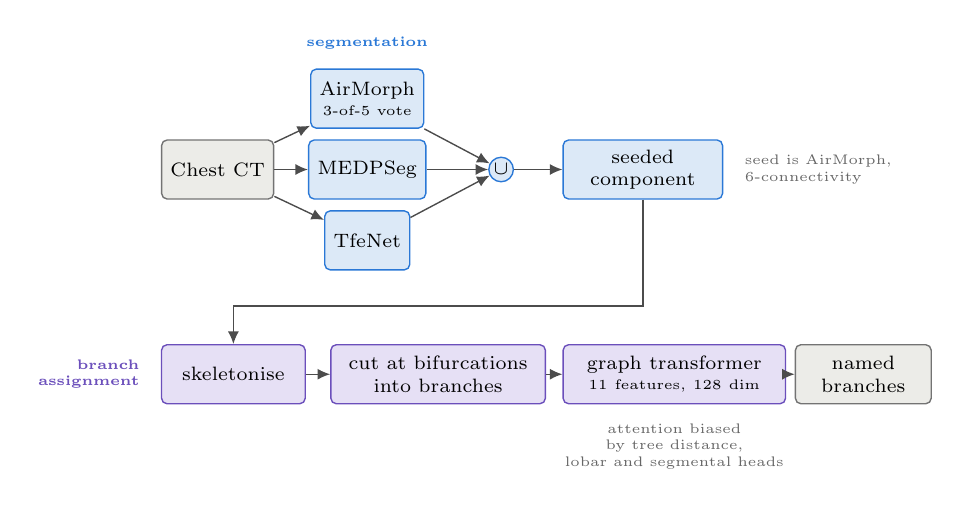
\begin{tikzpicture}

% ---- row 1, the segmentation front end
\node[io] (ct) {Chest CT};
\node[seg] (mp) at ($(ct)+(19mm,0)$) {MEDPSeg};
\node[seg] (am) at ($(mp)+(0,9mm)$) {AirMorph\\[-1pt]\tiny 3-of-5 vote};
\node[seg] (tf) at ($(mp)+(0,-9mm)$) {TfeNet};
\node[op]  (or) at ($(mp)+(17mm,0)$) {$\cup$};
\node[seg, text width=18mm] (lcc) at ($(or)+(18mm,0)$) {seeded\\component};
\node[note, right=1.5mm of lcc, text width=21mm, align=left]
  {seed is AirMorph,\\6-connectivity};
\draw[fl] (ct) -- (am); \draw[fl] (ct) -- (mp); \draw[fl] (ct) -- (tf);
\draw[fl] (am) -- (or); \draw[fl] (mp) -- (or); \draw[fl] (tf) -- (or);
\draw[fl] (or) -- (lcc);

% ---- row 2, branch assignment. The connector runs in a clear channel between
% the rows, so it crosses no block.
\node[lab, text width=16mm] (sk) at ($(ct)+(2mm,-26mm)$) {skeletonise};
\node[lab, text width=25mm] (pc) at ($(sk)+(26mm,0)$) {cut at bifurcations\\into branches};
\node[lab, text width=26mm] (gt) at ($(pc)+(30mm,0)$)
  {graph transformer\\[-1pt]\tiny 11 features, 128 dim};
\node[io, text width=15mm] (out) at ($(gt)+(24mm,0)$) {named\\branches};
\draw[fl] (sk) -- (pc); \draw[fl] (pc) -- (gt); \draw[fl] (gt) -- (out);
\node[note, below=1.2mm of gt, text width=32mm]
  {attention biased by tree distance,\\lobar and segmental heads};

\coordinate (ch) at ($(lcc.south)+(0,-13.5mm)$);
\draw[fl] (lcc.south) -- (ch) -| (sk.north);

% ---- which stage is which
\node[note, above=1.2mm of am, text width=30mm, text=segline]
  {\textbf{segmentation}};
\node[note, left=1.5mm of sk, text width=13mm, align=right, text=labline]
  {\textbf{branch\\assignment}};
\end{tikzpicture}
\caption{The pipeline as blocks. One chest CT is segmented independently by
three public models, their masks are combined by a bitwise union, and a single
connected component is retained by seeding it from the AirMorph mask rather than
by taking the largest one. That mask is skeletonised, the skeleton is cut at
bifurcations into branches, and a graph transformer names each branch from its
geometry and its position in the tree. Figure~\ref{fig:pipeline} shows the same
stages as images on one examination.}
\label{fig:arch}
\end{figure}

\begin{figure}[tbp]
\centering
\includegraphics[width=\textwidth]{figures/03_pipeline.pdf}
\caption{The pipeline on one examination, the 0.9-year-old infant used
throughout. \textbf{(a) Computed tomography}, as a minimum intensity projection
through the same slab as the renders beside it, so that the airway lumen reads
as a dark tree against aerated lung. \textbf{(b) Airway segmentation}, the
three-model union under seeded component selection. \textbf{(c) Centreline}.
\textbf{(d) Branch parcellation}, the centreline cut at bifurcations into 164
branches, each in its own colour, which are the nodes the graph transformer
receives. \textbf{(e) Anatomical assignment}, the predicted label of every
branch painted back onto the airway surface. Branches proximal to the lobar
division carry the tracheal class, which is how the annotation vocabulary treats
them. Panels (b) to (e) share one crop, camera and light, so only the
representation changes.}
\label{fig:pipeline}
\end{figure}

\subsection{Segmentation}
Figure~\ref{fig:pipeline} shows the whole pipeline on one examination. Three
airway models are run independently and their binary masks combined by a bitwise
OR. Component pruning is applied once, to the union, rather than to each member,
because a detached distal fragment from one member is precisely what another
member's mask is meant to reconnect. The retained component is the one
containing the most voxels of a designated seed member, under
6-connectivity.\footnote{Common libraries encode this as
\texttt{connectivity}~$=1$, where 2 and 3 denote the 18- and 26-neighbourhood.}
Selecting by size instead fails when a member emits a component larger than the
airway and disjoint from it, which is the failure quantified in
Section~\ref{sec:res-selection}. If the seed does not intersect the union the
rule falls back to the largest component.

Figure~\ref{fig:panels} shows the stage in detail. Two members are released
checkpoints \cite{carmo2024medpseg,wu2025tfenet} and the seed is a
three-of-five vote of architectures trained on the 239-volume split. Source volumes are LAS and two of the three models ignore direction
cosines, so reorientation is applied in both directions and verified
quantitatively by sampling the original CT at the final mask voxels, which must
return air density.

\subsection{Branch assignment}
The fused mask is skeletonised, the skeleton is cut into segments at bifurcation
voxels, every lumen voxel is assigned to its nearest segment, and a
parent-child tree is built. Generation is depth from the root plus one, so the
trachea is generation 1. Other conventions number differently.

Each segment becomes a graph node carrying 11 geometric features, and a graph
transformer with 128 hidden dimensions predicts a lobar, a segmental and a
subsegmental label per node, with attention biased by tree distance
\cite{zhang2025airmorph}. The weights were not released, so the network was
trained here and the choices the published description leaves open are stated
explicitly. The optimiser follows the published Adam at $5\times10^{-4}$. No
labelling loss is given, and cross-entropy with deep supervision over the heads
was adopted. The stated 32 attention heads contradict the released configuration
of four heads of dimension 32, and the configuration was followed so the trained
weights load into the released inference path unchanged. Training ran 600 epochs
with validation every 10, one graph per step, and the exported checkpoint is the
best validation epoch by the surrogate accuracy described next, 559 of 600. The
run took three hours and seven minutes on one GPU.

Of the 6 lobar, 20 segmental and 82 subsegmental heads only the first two are
supervised by real labels. The public annotations are a 20-value segmental
scheme, verified at the data, and no subsegmental reference was released, so the
subsegmental head was trained toward the base subsegment of each segment. Its
accuracy is therefore segment granularity expressed in subsegmental identifiers
and is not a subsegmental result, and we report lobar and segmental accuracy
only. This differs from \cite{zhang2025airmorph}, whose 127 subsegmental classes
come from a private annotation set. The inference path offers no abstention, so
a non-root branch predicted as tracheal at every level is flagged rather than
reported as anatomy.

\subsection{Evaluation}
Metric definitions differ between publications and are stated as implemented.
With $P$ the predicted and $G$ the reference airway voxels, DSC is
$2|P\cap G|/(|P|+|G|)$, precision $|P\cap G|/|P|$ and sensitivity
$|P\cap G|/|G|$. Tree length detected (TLD) is $|S_G \cap P|/|S_G|$ on the
reference centerline $S_G$, and clDice \cite{cldice} is the harmonic mean of
$|S_P\cap G|/|S_P|$ and $|S_G\cap P|/|S_G|$. A branch is detected (BND) when at
least 80 per cent of its reference centerline voxels lie inside $P$. TLD and BND
are voxel-count fractions with no spacing weighting, so a subsegmental
centerline voxel counts as much as a tracheal one. For per-generation
evaluation every reference voxel inherits the generation of its branch and
metrics are recomputed with the reference restricted to one generation, the
prediction left unrestricted, and predicted voxels attributed by the same
nearest-branch map. Pooling all generations reproduces the whole-tree values on
every case.


\begin{figure}[tbp]
\centering
\includegraphics[width=\textwidth]{figures/01_member_panels.pdf}
\caption{The segmentation stage on one examination, an infant of 0.9 years.
Every panel shares one crop, camera and physical scale, so what differs is the
mask alone, and the frame is set by the union so that nothing any member
produced is cropped away. AirMorph (a) is conservative and clean, MEDPSeg (b)
adds detached debris, and TfeNet (c) contributes two slab artefacts that
together exceed the airway in volume. Their union (d) inherits all of it.
Selecting the component carrying the seed rather than the largest one recovers
the airway (e). On this examination the largest component is a slab, so the
conventional rule would have discarded the tree entirely. Panel (e) is rendered
on a finer grid with smoothing artefacts suppressed, which does not affect the
volumes printed on the panels, measured on the masks themselves.}
\label{fig:panels}
\end{figure}

% =====================================================================
\section{Results}
\label{sec:results}

\subsection{Combination strategy}
Table~\ref{tab:variants} reports each model alone and every combination of them
on the benchmark test set. The two families of metric do not agree. Majority
voting attains the highest DSC, precision and surface distance, while the union
of all three members attains the highest TLD, BND and sensitivity. Every
combination sits between 1.43 and 1.82 mm of surface distance, under two voxels,
and the difference between the union and the best of them is not significant. We adopt the union,
because completeness governs whether a branch can be labelled at all, whereas a
branch recovered with a slightly inaccurate boundary can still be named.

The three models differ sharply in character. MEDPSeg is conservative and
accurate, at DSC 93.29 and precision 92.02, but detects only 76.10 per cent of
branches. TfeNet sits at the other extreme, at precision 53.68 and DSC 65.23,
and is no more complete for being permissive, reaching BND 75.65 against
MEDPSeg's 76.10. It still contributes, because what it adds is not what the
other two already hold. AirMorph is the strongest single model on topology at
BND 91.27 and the union improves on it by a full point. Within AirMorph one
member reaches TLD 95.40 alone, above the union's 95.22, while the union leads
on branch detection at 92.31 against that member's 91.68.

Whether that trade can be avoided was tested before settling on the union.
Fifty-one combination rules were scored on the 30 validation volumes, and none
dominated the union across all six metrics on either split. One rule does lead
four columns on test, but by admitting almost everything, at DSC 77.07 and
precision 63.53 against the union's 93.06 and 88.71. Completeness and boundary
agreement trade against each other here, and we take the completeness side
because that is what the next stage depends on.

\begin{table}[tbp]
\centering
\caption{Each model alone and every combination of them, on the 30 held-out
benchmark volumes. Component selection is the seeded rule throughout, and the
individual models are scored as the combination consumes them, before their own
post-processing. The strategy adopted for the rest of the paper is the union of
all three members, for the reason given in the text. HD95 is the 95th
percentile of the surface distance in millimetres, which the plain Hausdorff
distance cannot replace here because a single voxel sets it. Best value per
column in bold, second best underlined.}
\label{tab:variants}
\setlength{\tabcolsep}{3.5pt}\footnotesize
\begin{tabular}{@{}lccccccc@{}}
\toprule
Strategy & DSC & clDice & TLD & BND & Sens. & Prec. & \hd{HD95\\(mm)} \\
\midrule
AirMorph & 91.64 & 89.05 & \underline{94.95} & 91.27 & 95.04 & 89.12 & 2.77 \\
MEDPSeg & 93.29 & 85.82 & 87.50 & 76.10 & 94.78 & 92.02 & 2.36 \\
TfeNet & 65.23 & 51.03 & 86.54 & 75.65 & 91.44 & 53.68 & 133.70 \\
\midrule
AirMorph $\cup$ MEDPSeg & 93.15 & 90.32 & 94.44 & 91.29 & \underline{98.06} & 88.99 & 1.66 \\
AirMorph $\cup$ TfeNet & 93.29 & \textbf{90.81} & 94.80 & \underline{91.61} & 97.43 & 89.83 & 1.75 \\
MEDPSeg $\cup$ TfeNet & \underline{94.08} & 90.06 & 88.96 & 81.91 & 95.96 & 92.55 & \underline{1.64} \\
All three members & 93.06 & 90.24 & \textbf{95.22} & \textbf{92.31} & \textbf{98.23} & 88.71 & 1.81 \\
\midrule
Majority vote & 94.04 & 89.63 & 90.94 & 83.19 & 95.51 & \underline{93.07} & 1.82 \\
Majority vote, selected & \textbf{94.38} & \underline{90.48} & 87.84 & 80.35 & 95.00 & \textbf{94.04} & \textbf{1.43} \\
\bottomrule
\end{tabular}
\end{table}

\subsection{Component selection}
\label{sec:res-selection}
Replacing the seeded rule with largest-component selection affected three of the
four union strategies, each on the same three examinations, where the retained
mask had no overlap at all with the reference and every metric scored zero.
Across the four unions this is 9 of 120 pairs, with the same component retained
on the remaining 111, and the union without the permissive member was never
affected, consistent with the mechanism. On the three affected examinations the
retained component measured 242\,471, 126\,664 and 128\,539 voxels against the
true airway's 198\,567, 122\,161 and 97\,738. At test-set level the effect is a
change in dispersion rather than a uniform loss. Mean DSC for the union of all
three falls from 93.06 to 84.57 while the standard deviation rises from 4.37 to
28.74, so the distribution is bimodal rather than degraded.

In children the rule matters far more. Across 83 screened pediatric
examinations the two rules disagreed on six, and every one was an infant under
one year of age, six of the nine such examinations present, while they agreed on
all 74 aged one year and above. The comparable adult figure is three of 30.

\subsection{Accuracy by generation}
Table~\ref{tab:gen} and Figure~\ref{fig:gen} report accuracy generation by
generation. The whole-tree
DSC of 93.06 describes no generation well, falling from 98.39 at the trachea to
74.73 at generation 10 and dropping below 90 by generation 6. The decline is
driven by precision, 97.33 to 69.17, far more than by sensitivity, 99.50 to
89.89, so peripherally the method finds the branch and disagrees about its
boundary. Branch detection degrades more slowly, remaining at 91.04 per cent at
generation 7 where DSC has already fallen to 80.06, so tree structure survives
further into the periphery than voxel agreement does. Dispersion widens sharply,
with the standard deviation of DSC rising from 1.07 to 19.76.

\begin{figure}[tbp]
\centering
\includegraphics[width=\textwidth]{figures/04_by_generation.pdf}
\caption{Accuracy against airway depth on the benchmark test set. Left, the
asymmetry the paper turns on. Segmentation falls steeply with generation and
naming does not, so once a branch has been recovered it is named reliably and
the periphery is a segmentation problem rather than a labelling one. The band is
one standard deviation of Dice across volumes, and it widens with depth as much
as the mean falls. Sensitivity and branch detection fall far more slowly than
Dice and precision, which is the same observation from the other side: the tree
structure survives deeper than voxel agreement does. The naming curves are drawn
flat past generation 7 because the annotation pools everything beyond it into
one bin. Right, the reference branches by generation. Most of them lie where accuracy has already dropped,
which is why a whole-tree mean flatters the method and why accuracy is reported
per generation here.}
\label{fig:gen}
\end{figure}

\begin{table}[tbp]
\centering
\caption{Accuracy by airway generation on the benchmark test set, union of all
three members, over the volumes containing each generation.}
\label{tab:gen}
\setlength{\tabcolsep}{4pt}\footnotesize
\begin{tabular}{@{}lccccc@{}}
\toprule
Gen & \hd{Ref.\\branches} & \hd{Volumes\\present} & DSC & Sensitivity & Precision \\
\midrule
1  & 30   & 30 & $98.39\pm1.07$ & $99.50\pm0.75$ & $97.33\pm2.12$ \\
2  & 66   & 30 & $97.92\pm1.32$ & $99.44\pm0.98$ & $96.49\pm2.58$ \\
3  & 128  & 30 & $96.80\pm3.08$ & $98.98\pm1.72$ & $94.94\pm5.67$ \\
4  & 262  & 30 & $94.70\pm4.44$ & $98.73\pm2.01$ & $91.36\pm7.59$ \\
5  & 542  & 30 & $90.40\pm8.05$ & $98.22\pm3.27$ & $84.70\pm11.80$ \\
6  & 985  & 30 & $85.38\pm9.89$ & $96.51\pm4.06$ & $77.89\pm13.55$ \\
7  & 1482 & 30 & $80.06\pm11.43$ & $94.23\pm6.59$ & $71.28\pm15.23$ \\
8  & 1444 & 29 & $80.66\pm9.74$ & $94.58\pm5.23$ & $71.83\pm13.85$ \\
9  & 1008 & 29 & $79.37\pm11.84$ & $94.39\pm6.85$ & $70.70\pm16.05$ \\
10 & 593  & 29 & $74.73\pm19.76$ & $89.89\pm16.74$ & $69.17\pm20.23$ \\
\midrule
\multicolumn{3}{@{}l}{Whole tree, pooled} & $93.06\pm4.37$ & $98.23\pm1.56$ & $88.71\pm7.08$ \\
\bottomrule
\end{tabular}
\end{table}

\subsection{Branch assignment}
Table~\ref{tab:label} reports assignment on the 11 held-out annotated volumes in
two settings. The first parses the graph from the reference airway, so the node
set is the reference node set and every branch is scorable. This isolates the
labelling network from segmentation error and gives 99.34 per cent lobar and
97.01 per cent segmental accuracy.

The second setting is the deployed path, where the graph is parsed from the
predicted mask. Accuracy is almost unchanged, at 99.37 and 97.07 per cent, but
it is measured over a different node set and the two are not the same quantity.
A predicted branch lying outside the annotated tree has no reference label and
cannot be scored, and 86.8 per cent of predicted branches have a counterpart.
The unscorable remainder is not counted as a labelling error, which is why the
scorable fraction is reported beside the accuracy rather than folded into it.
Its spread across volumes is wide, from 56.3 to 99.4 per cent, and it is the
quantity that limits what the deployed pipeline can be said to name.

Segmental accuracy varies far more than lobar, with a worst volume at 87.98 per
cent against a lobar worst of 98.15. Topological consistency, the fraction of
branches whose predicted name agrees with the names of their descendants, is
98.95 per cent and is label free, so it can be computed where no reference
exists.

Per branch, over the 2849 reference branches of the 11 volumes, lobar accuracy
is 99.43 and segmental accuracy 97.35 per cent, and the behaviour with depth is
the opposite of segmentation. Generations 1 to 3 are named without error and
accuracy is essentially flat thereafter, at 97.50 segmental at generation 7 and
96.88 beyond it, against a segmentation Dice that has fallen from 98.39 to 80.06
over the same range (Table~\ref{tab:gen}). Naming a branch is therefore not the
limiting step once the branch has been recovered. The segmental errors
concentrate in the basal segments, where the four weakest classes of reasonable
size fall to between 88 and 91 per cent, and in the branches the annotation
leaves proximally unnamed, at 94.71 per cent lobar.

\begin{table}[tbp]
\centering
\caption{Branch assignment on the 11 held-out annotated volumes, mean $\pm$ SD.
Reference graphs isolate the labelling network, predicted graphs are the
deployed path. Accuracies are computed over scorable branches only.}
\label{tab:label}
\setlength{\tabcolsep}{5pt}\footnotesize
\begin{tabular}{@{}lcccc@{}}
\toprule
Graph source & \hd{Branches\\scorable (\%)} & \hd{Lobar\\accuracy} &
\hd{Segmental\\accuracy} & \hd{Segmental\\TreeCons} \\
\midrule
Reference  & 100 & $99.34\pm0.68$ & $97.01\pm3.82$ & $98.95\pm1.69$ \\
Predicted  & $86.75\pm17.03$ & $99.37\pm0.69$ & $97.07\pm5.82$ & $98.92\pm1.56$ \\
\bottomrule
\end{tabular}
\end{table}

\subsection{Pediatric benchmark}
Table~\ref{tab:ped} repeats the comparison of Table~\ref{tab:variants} on the
nine annotated pediatric volumes. The union leads six of the seven metrics. It
detects 86.40 per cent of reference branches against 80.36 for the best pair,
recovers 93.91 per cent of reference tree length against 90.58, and reaches
sensitivity 90.21 against 88.85, and has the smallest surface distance at
0.53 mm. Only precision is higher elsewhere, by one part in a thousand.

The margins are what separates this table from the adult one. On the adult
benchmark the union leads branch detection by 0.7 points. Here it leads by 6.0.
Combining models is worth roughly an order of magnitude more in children than in
adults, which is the case for the front end this paper adopts. Dispersion is
also far wider, with per-case branch detection running from 70.5 to 99.0 per
cent, so a single pediatric mean describes the method less well than an adult
mean does.

\begin{table}[tbp]
\centering
\caption{Each model alone and every combination of them on the nine annotated
pediatric volumes, seeded selection, mean over volumes. HD95 is the 95th
percentile of the surface distance in millimetres. Best value per column in
bold, second best underlined.}
\label{tab:ped}
\setlength{\tabcolsep}{3.5pt}\footnotesize
\begin{tabular}{@{}lccccccc@{}}
\toprule
Strategy & DSC & clDice & TLD & BND & Sens. & Prec. & \hd{HD95\\(mm)} \\
\midrule
AirMorph & 88.54 & 92.56 & 84.01 & 69.51 & 79.64 & 99.89 & 1.35 \\
MEDPSeg & 80.40 & 74.51 & 76.60 & 53.17 & 83.20 & 80.83 & 44.86 \\
TfeNet & 49.95 & 26.37 & 83.58 & 66.85 & 83.31 & 38.05 & 118.81 \\
\midrule
AirMorph $\cup$ MEDPSeg & \underline{94.01} & 95.39 & 89.46 & 77.01 & \underline{88.85} & \underline{99.90} & \underline{0.54} \\
AirMorph $\cup$ TfeNet & 93.06 & \underline{95.61} & \underline{90.58} & \underline{80.36} & 87.20 & 99.87 & 0.55 \\
MEDPSeg $\cup$ TfeNet & 93.39 & 94.57 & 87.36 & 74.10 & 87.77 & 99.87 & \underline{0.54} \\
All three members & \textbf{94.74} & \textbf{97.06} & \textbf{93.91} & \textbf{86.40} & \textbf{90.21} & 99.85 & \textbf{0.53} \\
\midrule
Majority vote & 88.15 & 87.54 & 82.50 & 60.78 & 84.03 & 93.64 & 13.02 \\
Majority vote, selected & 90.93 & 91.49 & 80.17 & 59.26 & 83.48 & \textbf{99.95} & 0.85 \\
\bottomrule
\end{tabular}
\end{table}

The residual error is of a benign kind. Of the reference material the method
does not recover, 97.7 per cent lies within one voxel of the predicted surface,
so what is missed is mostly calibre at the boundary rather than whole branches.

Over the 90-examination cohort, median airway volume across generations 1 to 10
rises monotonically from 3.0 to 39.7 mL and median intrathoracic tracheal length
from 36.6 to 107.8 mm across the nine age bands, and nothing in the pipeline
enforces that ordering. Per-generation diameter correlates with age at every
generation, with Spearman coefficients between 0.82 and 0.95, all $p<0.001$.
\todo{if a supplement is submitted, point here to the per-generation
morphometry tables}

% =====================================================================
\section{Discussion and Conclusion}

The two stages fail in opposite ways with depth, and that asymmetry is the main
practical finding. Segmentation degrades steeply while labelling stays near
flat, so once a branch is recovered it is named reliably. What limits the
deployed pipeline is the periphery the segmentation never recovers, together
with the 13.3 per cent of predicted branches that have no annotated counterpart
and therefore cannot be verified at all. Effort is better spent on segmentation
completeness and on extending the reference standard than on the labelling
network.

The peripheral decline is a resolution limit rather than a modelling failure.
Boundary disagreement is a small fraction of a proximal airway and a large
fraction of a distal one, which sets a ceiling for a given voxel size. An
anatomical branch is physically smaller in a child, so it reaches that regime at
a shallower generation. The adult decline reported here is therefore an
optimistic bound on the pediatric case. The component-selection result is
where the two settings diverge most. Largest-component selection is standard and
nearly harmless in adults, at three of 30, but altered six of 83 pediatric
examinations and every one was an infant, six of nine. A method validated only
in adults would not have surfaced this.

\smallskip\noindent\textbf{Limitations.}
One segmentation member was trained on the public
annotation pool from which the benchmark test volumes are drawn, so values
involving it are upper bounds, although the union of the two unexposed members
retains the same ordering. Evaluation stops at a fixed generation and no claim
is made beyond it. Tortuosity and calibre variability depend on how many voxels
a branch spans. Ten examinations per age band describe the cohort and do not
establish reference limits. The segmentation is lumen only, so wall thickness
and bronchus-artery ratios are out of scope.

\subsubsection*{Acknowledgements.} \todo{Acknowledgements and funding.}

\subsubsection*{Disclosure of interests.} \todo{Competing interests statement.}

\bibliographystyle{splncs04}
\bibliography{airway_method_paper}

\end{document}
